\documentclass{beamer}
\usepackage[utf8]{inputenc}

\usetheme{Madrid}
\usecolortheme{default}
\usepackage{amsmath,amssymb,amsfonts,amsthm}
\usepackage{mathtools}
\usepackage{txfonts}
\usepackage{tkz-euclide}
\usepackage{listings}
\usepackage{adjustbox}
\usepackage{array}
\usepackage{gensymb}
\usepackage{tabularx}
\usepackage{gvv}
\usepackage{lmodern}
\usepackage{circuitikz}
\usepackage{tikz}
\lstset{literate={·}{{$\cdot$}}1 {λ}{{$\lambda$}}1 {→}{{$\to$}}1}
\usepackage{graphicx}

\setbeamertemplate{page number in head/foot}[totalframenumber]

\usepackage{tcolorbox}
\tcbuselibrary{minted,breakable,xparse,skins}



\definecolor{bg}{gray}{0.95}
\DeclareTCBListing{mintedbox}{O{}m!O{}}{%
  breakable=true,
  listing engine=minted,
  listing only,
  minted language=#2,
  minted style=default,
  minted options={%
    linenos,
    gobble=0,
    breaklines=true,
    breakafter=,,
    fontsize=\small,
    numbersep=8pt,
    #1},
  boxsep=0pt,
  left skip=0pt,
  right skip=0pt,
  left=25pt,
  right=0pt,
  top=3pt,
  bottom=3pt,
  arc=5pt,
  leftrule=0pt,
  rightrule=0pt,
  bottomrule=2pt,
  toprule=2pt,
  colback=bg,
  colframe=orange!70,
  enhanced,
  overlay={%
    \begin{tcbclipinterior}
    \fill[orange!20!white] (frame.south west) rectangle ([xshift=20pt]frame.north west);
    \end{tcbclipinterior}},
  #3,
}
\lstset{
    language=C,
    basicstyle=\ttfamily\small,
    keywordstyle=\color{blue},
    stringstyle=\color{orange},
    commentstyle=\color{green!60!black},
    numbers=left,
    numberstyle=\tiny\color{gray},
    breaklines=true,
    showstringspaces=false,
}
\title{Problem 2.2.28}
\author{Sujal Rajani}

\date{\today} 
\begin{document}

\begin{frame}
\titlepage
\end{frame}



\begin{frame}{Question}
\textbf{Question}:
\noindent Find the angle between the two planes 2x+y-2z=5 and 3x-6y-2z=7 using vector method.
\end{frame}

\begin{frame}{Solution}
\textbf{Solution:} 
\\
 the   normal vector of plane 2 x+y-2z=5 is : $\vec{n_1}$
 \begin{align*}
     \vec{n_1}=\myvec{2\\1\\-2}
 \end{align*}
 the normal vector of plane 3 x-6y-2z=7 is : $\vec{n_2}$
 \begin{align*}
     \vec{n_2}=\myvec{3\\-6\\-2}
 \end{align*} 
 The value of $||\vec{n_1}||$:
  \begin{align*}
     (\vec{n_1})^T(\vec{n_1})={||\vec{n_1}||}^2=9
 \end{align*}
 \end{frame} 
 
 \begin{frame}{SOLUTION}
 The value of $||\vec{n_2}||$:
  \begin{align*}
     (\vec{n_2} )^T(\vec{n_2})={||\vec{n_2}||}^2=49
 \end{align*}
 The angle between two plane is same as the angle between their normal vectors , which is  $\theta$ .
\\
\\
 the angle between $\vec{n_1}$ and $\vec{n_2}$ is :
 \begin{align*}
      \cos{\theta} = \dfrac{(\vec{n_1})^T(\vec{n_2})}{||\vec{n_1}||\quad||\vec{n_2}||}=\dfrac{4}{21}
       \\
      \theta=cos^{-1}\dfrac{4}{21}
 \end{align*}
 \end{frame}


       \begin{frame}[fragile]
    \begin{figure}[H]
    \centering
    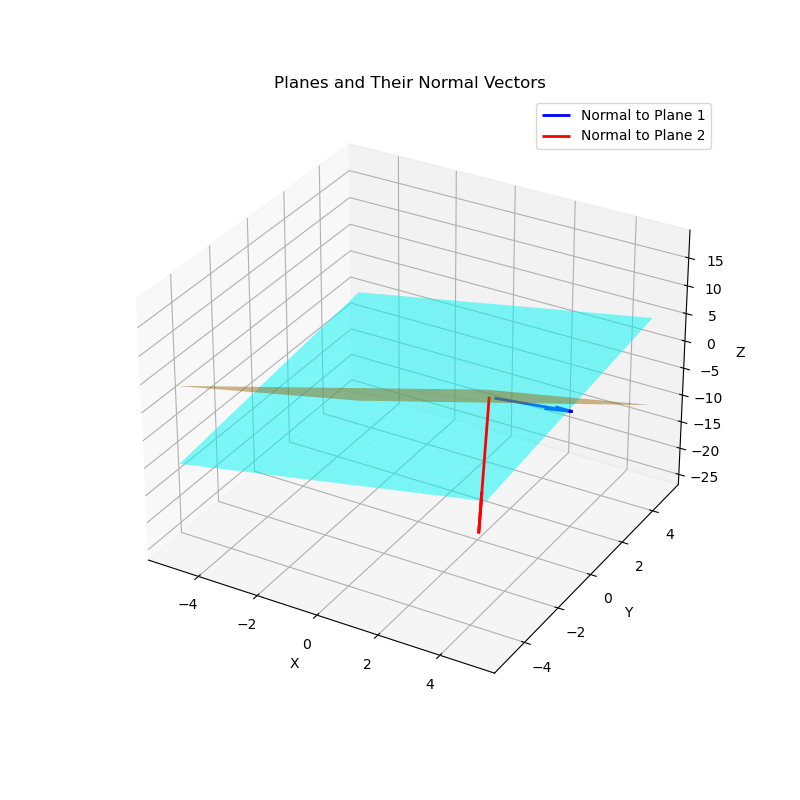
\includegraphics[width = 0.6\columnwidth]{../figs/img.png}
    \caption*{}
    \label{figs}
\end{figure}
\end{frame}
\section{ C Code}
\begin{frame}[fragile]
\frametitle{C Code }
\begin{lstlisting}[language=C]
#include <stdio.h>
#include <math.h>

// Function to compute dot product
double dot(double a[3], double b[3]) {
    return a[0]*b[0] + a[1]*b[1] + a[2]*b[2];
}

// Function to compute magnitude of a vector
double magnitude(double v[3]) {
    return sqrt(v[0]*v[0] + v[1]*v[1] + v[2]*v[2]);
}

int main() {
    // Normal vectors of the two planes
    double n1[3] = {2, 1, -2};   // for plane 2x + y - 2z = 5
    double n2[3] = {3, -6, -2};  // for plane 3x - 6y - 2z = 7

 
\end{lstlisting}
\end{frame}

\begin{frame}[fragile]
\frametitle{C Code }
\begin{lstlisting}[language=C]
 // Dot product
    double dot_val = dot(n1, n2);
    // Magnitudes
    double mag1 = magnitude(n1);
    double mag2 = magnitude(n2);

    // Cos(theta)
    double cos_theta = dot_val / (mag1 * mag2);

    // Angle in radians and degrees
    double theta_rad = acos(cos_theta);
    double theta_deg = theta_rad * 180.0 / M_PI;

   

    
\end{lstlisting}
\end{frame}
\begin{frame}[fragile]
\frametitle{C Code }
\begin{lstlisting}[language=C]
 // Output
    printf("Dot product = %.2f\n", dot_val);
    printf("|n1| = %.2f, |n2| = %.2f\n", mag1, mag2);
    printf("cos(theta) = %.4f\n", cos_theta);
    printf("Angle between planes = %.4f radians = %.2f degrees\n", theta_rad, theta_deg);

    return 0;
}
\end{lstlisting}
\end{frame}
\begin{frame}[fragile]
\frametitle{Python Code for Plotting}
\begin{lstlisting}[language=Python]
import sympy as sp
import numpy as np
import matplotlib.pyplot as plt
import matplotlib as mp
mp.use("TkAgg")

# ------------------------
# Step 1: Define planes
# ------------------------
n1, d1 = sp.Matrix([2, 1, -2]), 5            # 2x + y - 2z = 5
n2, d2 = sp.Matrix([3, -6, -2]), 7           # 3x - 6y - 2z = 7

# ------------------------
# Step 2: Function to plot a plane
# ------------------------
def plot_plane(ax, n, d, color, alpha=0.4):
    xx, yy = np.meshgrid(np.linspace(-5,5,15), np.linspace(-5,5,15))
    zz = (d - n[0]*xx - n[1]*yy) / n[2]
    ax.plot_surface(xx, yy, zz, color=color, alpha=alpha)

\end{lstlisting}

\end{frame}
\section{Python Code}
\begin{frame}[fragile]
\frametitle{Python Code for Plotting}
\begin{lstlisting}[language=Python]   
# ------------------------
# Step 3: Get points on planes for plotting normals
# ------------------------
x, y, z = sp.symbols('x y z')
plane1_eq = n1[0]*x + n1[1]*y + n1[2]*z - d1
plane2_eq = n2[0]*x + n2[1]*y + n2[2]*z - d2

p1 = sp.solve(plane1_eq.subs({y:0, z:0}), x)
p2 = sp.solve(plane2_eq.subs({y:0, z:0}), x)

a1 = np.array([float(p1[0]), 0, 0]) if p1 else np.zeros(3)
a2 = np.array([float(p2[0]), 0, 0]) if p2 else np.zeros(3)

# ------------------------
# Step 4: Plot planes + normals
# ------------------------
fig = plt.figure(figsize=(8,8))
ax = fig.add_subplot(111, projection='3d')

n1f, d1f = np.array([float(v) for v in n1]), float(d1)
n2f, d2f = np.array([float(v) for v in n2]), float(d2)


\end{lstlisting}

\end{frame}
\begin{frame}[fragile]
\frametitle{Python Code for Plotting}
\begin{lstlisting}[language=Python]   

plot_plane(ax, n1f, d1f, "cyan", 0.5)
plot_plane(ax, n2f, d2f, "orange", 0.5)

# Plot normal vectors
ax.quiver(a1[0], a1[1], a1[2], n1f[0], n1f[1], n1f[2],
          length=3, color="blue", linewidth=2, label="Normal to Plane 1")
ax.quiver(a2[0], a2[1], a2[2], n2f[0], n2f[1], n2f[2],
          length=3, color="red", linewidth=2, label="Normal to Plane 2")

# Labels
ax.set_xlabel("X")
ax.set_ylabel("Y")
ax.set_zlabel("Z")
ax.set_title("Planes and Their Normal Vectors")
ax.legend()

plt.show()

\end{lstlisting}

\end{frame}
\end{document}